\chapter{L'exploitation des informations via des failles}

A la suite de la phase de récupération d'informations, nous allons chercher des failles au sein de la machine cible. Certains outils de la précédente étape ont déjà pu nous aiguiller sur le type de failles à exploiter. Nous allons donc vous expliquer dans cette partie quelles sont les principales failles de sécurités que vous pourriez rencontrer et comment les exploiter.

\section{Le déni de services}

Actuellement, le déni de services(DoS) ou  déni de service distribué (DDoS) est utilisé afin de paralyser un réseau ou un site web pour plusieurs raisons et cela peut vite coûter chère. Cependant, bloquer un service signifie mobiliser du personnel de sécurité afin de résoudre le problème et donc, réduire l'attention sur un autre service qui lui présente des failles permettant une infiltration dans le réseau. Dans ce dossier, nous allons vous parler des DOS basés sur HTTP v2.

\subsection{Failles HTTP v2}

Avant d'expliquer en quoi consiste les failles HTTP v2, nous allons comprendre le fonctionnement de ce protocole.\\
Dans l'objectif de gagner en latence et en performance, HTTP v2 a été conçu et a réussi son pari. En effet, cette nouvelle version fait en sorte de réduire le nombre d'échanges entre un client et un serveur via le multiplexage de flux. De cette manière, un simple GET suffit pour obtenir une page Web. En plus de réduire le nombre d'échanges, HTTP v2 va compresser les entêtes HTTP et envoyer des contenus non-demandés qui seront stockés dans le cache (le Push) afin que le client puisse accéder beaucoup plus rapidement aux ressources. Malheureusement, tout ceci a permis l'ouverture au DOS. Nous allons vous en présenter trois qui sont :

\begin{itemize}
    \item \textbf{Slow Read Attack}
    \item \textbf{HPACK Bomb}
    \item \textbf{Dependency Cycle Attack}
\end{itemize}

Il en existe d'autres mais ces trois là ont été présentées lors de la Black Hat de 2016 et doivent donc être connues.

\subsubsection{Slow Read Attack}

Ce type d'attaque consiste à exploiter le protocole TCP à notre envie. En effet, dans TCP, il y a une "Window" qui consiste à dire au serveur notre capacité en réception de données. Ainsi, si nous réduisons la Window à une toute petite valeur et que nous le reproduisons plusieurs fois en même temps, notre programme va finir par laisser ouvert un certain nombre de sockets et ainsi créer de la latence voire même rendre le site indisponible. Pour effectuer ce DOS, le langage de programmation SCAPY peut être utilisé afin de modifier les requêtes.

\subsubsection{HPACK Bomb}

Comme nous l'avons vu plus haut, HTTP v2 compresse les entêtes HTTP sous forme binaire dans le but de gagner en ressource. Ce système se nomme le HPACK. L'attaque HPACK Bomb a pour but d'amplifier la taille du header car elle contient un tableau de taille dynamique ! Ainsi, nous pouvons rajoutons du contenu dans cette partie dynamique pour augmenter sa taille, jusqu'à obtenir la valeur de compression de base qui est de 4KB. Ensuite, grâce au mutliplexage de requêtes on va envoyer ce header 16 mille fois qui est le nombre maximal d'envoi en mutliplexage sur HTTP2. Un calcul rapide nous annonce qu'avec un envoi, le serveur va devoir décompresser 64 MB de données. La décompression comme la compression requièrent beaucoup de ressources au niveau de la RAM. Il ne reste alors plus qu'à faire une boucle en envoyant, en même temps, la plus grosse quantité de requêtes sur ce serveur avec ce header modifié et compressé afin d'effectuer un DOS.

\subsubsection{Dependency Cycle Attack}

La nouveauté de HTTP v2 est aussi le fait que le client puisse donner une priorité et un ordre aux éléments qui vont être traités par le serveur. Ce système se nomme "dependency". Chaque ordre a donc un numéro de priorité de ressources qui est associé à un numéro de mémoire. Ainsi, si deux éléments ont le même numéro de mémoire, le processus va reprendre son exécution à partir de ce point et donc créer une boucle infinie. Il est alors tout à fait imaginable de réaliser cette attaque couplée à un HPACK Bomb pour réaliser un très gros DOS.\\

Comme vous l'aurez compris, un DOS se base sur la structure des protocoles et peut attirer très vite l'attention de la sécurité informatique ciblé. Ces failles ne sont surtout pas à négliger lors de la réalisation d'une attaque.

\newpage

\section{Cookies}

\subsection{Généralités}

Il est désormais devenu courant de se retrouver face à ce message lorsque l’on souhaite entrer dans un site Web :

\begin{figure}[htp!]
  \centering
  \setlength\figureheight{7cm}
  \setlength\figurewidth{9cm}
  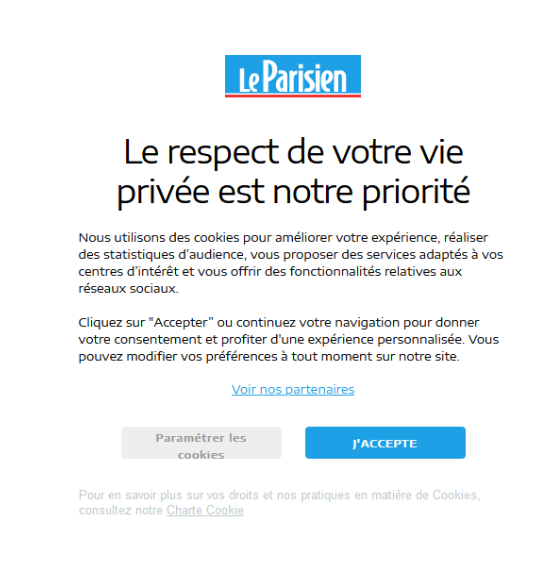
\includegraphics[width=1\textwidth]{oui/Ancien/imangeancien/cookie/cookie1.PNG}
   \caption{Utilisation des cookies sur le site Le Parisien}
  \label{fig:courbe-tikz}
\end{figure}

Cette page nous donne des informations concernant l’utilisation des cookies par le site Web et la possibilité qui nous est permise de pouvoir paramétrer l’utilisation de ces cookies. Force est de constater que la plupart du temps les utilisateurs qui se retrouvent face à cette page ignorent la signification d’un cookie et cliquent immédiatement sur accepter sans prendre le temps de se renseigner sur ce terme. En réalité, un cookie est une donnée envoyée par un serveur Web à votre navigateur. Ces données sont envoyées lorsque vous prenez la décision de visiter un site Web par exemple et cela permet au site en question de garder en mémoire des informations concernant vos habitudes de navigation, vos pseudos, vos mots de passe, vos paniers etc. Ces cookies sont stockés sur votre disque dur en tant que fichier. Ce fichier ne contient que du texte et est donc en principe totalement inoffensif. Malgré cela, certains logiciels antivirus nous mettent en garde contre des cookies provenant de certains sites. En d’autres termes, lorsque vous visitez un site ayant recours à des cookies, vous envoyez des informations à ce site afin qu’il soit en mesure d’améliorer votre expérience en vous proposant des services adaptés à vos centres d'intérêt. 

\subsection{Les différents types de cookies}

En règle générale, les cookies peuvent être soit temporaires, soit permanents. Les cookies temporaires sont désignés sous le terme de cookies de sessions et sont utilisés uniquement dans une session. Ces cookies sont supprimés lorsque l’on ferme notre navigateur. Les cookies permanents quant à eux sont utilisés dans différentes sessions de navigation et ils ne disparaissent que lorsque l’on décide de les supprimer ou bien lorsque leur dates d’expirations arrivent à terme. Parmi ces différents types de cookies, il existe les cookies dits internes et les cookies tiers. Les cookies internes sont mis en place par le site que vous consultez. Les cookies tiers quant à eux sont créés par un site différent de celui que vous consultez. Par exemple, de nombreux sites ont un bouton “J’aime” sur lequel on peut cliquer dessus. En cliquant sur ce bouton, un cookie pouvant être utilisé par Facebook s’activera.

\subsection{Mise en place d’un cookie}

\begin{figure}[htp!]
  \centering
  \setlength\figureheight{7cm}
  \setlength\figurewidth{9cm}
  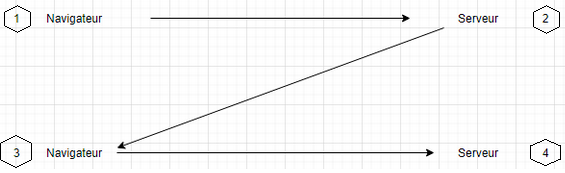
\includegraphics[width=0.7\textwidth]{oui/Ancien/imangeancien/cookie/cookie2.PNG}
   \caption{Transfert des cookies du navigateur au seveur}
  \label{fig:courbe-tikz}
\end{figure}

1. Le protocole HTTP permet de transférer des pages Web. A l’aide d’une requête HTTP, le navigateur appelle une page provenant du serveur Web.
Pour parvenir à la page www.velizy.fr/index.html, le navigateur se connecte au serveur www.velizy.fr en envoyant la requête suivante:
GET /index.html HTTP/1.0
Host: www.velizy.fr

2. Le serveur répond en transmettant au navigateur une réponse HTTP.
Cette réponse permet de demander au navigateur de conserver des cookies.
Afin de stocker un cookie, le serveur va ajouter dans la réponse HTTP une ligne Set-cookie. Cette ligne est en réalité une requête qui a pour but de demander au navigateur de stocker la chaîne nom=valeur.

3. Cette chaîne sera par la suite renvoyée dans toutes les prochaines requêtes envoyées au serveur s'il y a existence du cookie.
HTTP/1.0 200 OK
Content-type: text/html
Set-cookie: nom=valeur

\subsection{Durée de vie des cookies}

En théorie, tous les cookies ont un nom et une date d’expiration. 
Lorsque le site Web que vous consultez envoie un cookie, il prend l’initiative de demander à votre navigateur de stocker le cookie en question jusqu’à la date et l’heure inscrits dans le fichier texte. Il existe une loi dans laquelle il est stipulé que les cookies doivent être supprimés au moins une année après leur création. Malgré cela, certains cookies sont conservés bien plus longtemps. Pour l’anecdote, il est à savoir que des cookies ont été créés dans l’optique de durer 7000 ans.

\subsection{Interception des cookies}

Comme nous l’avons dit précédemment les cookies sont des données envoyées par un serveur web au navigateur de notre ordinateur. Or, les cookies peuvent contenir des informations que l’on qualifie de sensibles (pseudo, mot de passe). Par conséquent, il serait fort regrettable que quiconque puisse intercepter ces données.
Malheureusement, certaines méthodes permettent d’intercepter les cookies et nous allons ici en lister quelques unes.
La première méthode que nous allons expliquer se prénomme détournement de session. Cette attaque est essentiellement réalisée dans des lieux publics contenant des espaces WIFI non chiffré. Elle consiste en la lecture des communications d’autres utilisateurs sur le réseau en ayant recours à des "renifleurs de paquets". Cette lecture n’est possible que lorsque le trafic réseau n’est pas chiffré. En d’autres termes, pour éviter cette attaque, il suffit de chiffrer la connexion entre le serveur Web et l’ordinateur de l’utilisateur. Pour cela, on peut utiliser par exemple le protocole HTTPS.
La seconde méthode permettant d'intercepter des cookies est l’écriture de script directement dans les sites. Ces scripts ont pour but de demander au navigateur d’envoyer les cookies à des serveurs malveillants. Cette attaque est utilisée sur les sites qui permettent aux utilisateurs de publier du contenu HTML. Pour ce qui est de ce type d’attaque, chiffrer les cookies avant leur envoi sur le réseau n’a pas de grande utilité. En revanche afin de rendre inaccessible un cookie depuis l’exécution d’un script, il est possible d’utiliser le drapeau HttpOnly qui est une option introduite en 2002 sur le navigateur internet explorer.

\subsection{Protection contre le vol de cookie}

Le client d’un site Web n’a pas en sa possession de nombreux moyens permettant d’éviter qu’on intercepte ses cookies. En effet, il ne peut que prendre la décision de désactiver les cookies. Malheureusement, de nombreux sites Web ont recours à des cookies pour fonctionner convenablement.

Par conséquent, la sécurisation du vol de cookies est essentiellement à la charge du créateur du site Web. Il doit prendre en compte de nombreux détails afin de sécuriser au mieux son site et donc ses clients. Pour cela, le créateur du site Web doit éviter de stocker les données en lien avec l’authentification (pseudo ,mot de passe) en clair, mettre en place des identifiants de session aléatoires lors de chaque requête HTTP, effacer les cookies après leur utilisation. Il doit aussi chiffrer totalement, où au moins partiellement les cookies et surtout avoir recours à des protocoles sécurisés comme HTTPS.

\newpage

\section{Failles XSS (Cross-site scripting)}

Une faille XSS est une faille présente sur un site web qui permet l'exécution de code HTML ou JavaScript dans des variables mal protégées. Il ne faut pas confondre les failles XSS avec les failles SQL. En effet, la faille XSS s'exécute côté client sur le navigateur et non pas côté serveur sur une base de données par exemple.\\

\noindent Il existe deux types de failles XSS:

\begin{itemize}
    \item \textbf{Failles XSS réfléchies (non permanentes)}
    \item \textbf{Failles XSS stockées (permanentes)}
\end{itemize}

\noindent Nous verrons au cours de cette section ces deux types de failles, la structure d'une faille XSS ainsi que son utilisation par un pirate.

\subsection{XSS Reflected (réfléchies) }

La faille XSS non permanente est la faille la plus utilisée et sûrement la plus facile à pratiquer. En effet, l’attaquant n'a qu’à injecter du code dans l’input d’un formulaire et le faire apparaître à l’écran. Cette attaque ne nécessite donc en aucun cas un stockage contrairement au XSS stocké qui est présenté ci-dessous. Cette faille peut par exemple être présente lors de l'intervention d'un champ "rechercher" sur un site:

\begin{figure}[htp!]
  \centering
  \setlength\figureheight{7cm}
  \setlength\figurewidth{9cm}
  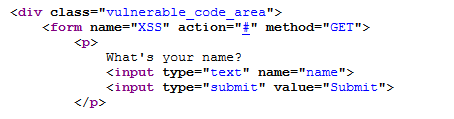
\includegraphics[width=0.6\textwidth]{oui/images/xss/xss.PNG}
  \caption{Code HTML recherche}
  \label{fig:courbe-tikz}
\end{figure}

\begin{figure}[htp!]
  \centering
  \setlength\figureheight{7cm}
  \setlength\figurewidth{9cm}
  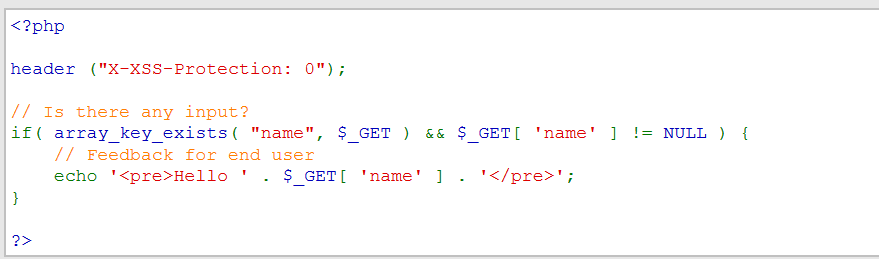
\includegraphics[width=0.9\textwidth]{oui/images/xss/xss2.PNG}
  \caption{Code PHP recherche}
  \label{fig:courbe-tikz}
\end{figure}

En regardant le code PHP, on peut s'apercevoir qu'il n'y a aucune vérification sur le paramètre \textbf{\$\_GET}. Cela veut dire que nous pouvons insérer n'importe quel code lors de la requête:

\begin{figure}[htp!]
  \centering
  \setlength\figureheight{7cm}
  \setlength\figurewidth{9cm}
  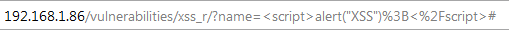
\includegraphics[width=0.8\textwidth]{oui/images/xss/xss4.PNG}
  \caption{Ajout code javascript}
  \label{fig:courbe-tikz}
\end{figure}

On constate à travers cette capture que notre script JS est passé en paramètre. On obtient donc la pop-up suvivante sur notre navigateur:\\

\begin{figure}[htp!]
  \centering
  \setlength\figureheight{7cm}
  \setlength\figurewidth{9cm}
  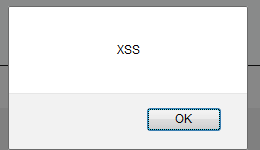
\includegraphics[width=0.3\textwidth]{oui/images/xss/xss3.PNG}
  \caption{Pop-up JS}
  \label{fig:courbe-tikz}
\end{figure}

Contrairement à ce que nous pourrions penser, le fait que la charge utile soit exécutée côté client est bel et bien un risque pour l’utilisateur. En effet, le client possède plusieurs informations secrètes et utiles pour l’attaquant, il a également des extensions dans son navigateur qui peuvent avoir des vulnérabilités.

Jusque-là, nous avons seulement affiché une pop-up dans la navigateur de la victime, mais nous allons aller un peu plus loin et voler les cookies de l’utilisateur sur le site vulnérable. Pour cela, nous utiliserons la propriété cookie du document (sous réserve que les cookies ne soient pas protégés):

\begin{center}
    \textbf{document.cookie}
\end{center}

\noindent En effet, si on exécute le code \lstinline{<script>alert(document.cookie);</script>} dans la barre de recherche du site on obtient la chose suivante:

\begin{figure}[htp!]
  \centering
  \setlength\figureheight{7cm}
  \setlength\figurewidth{9cm}
  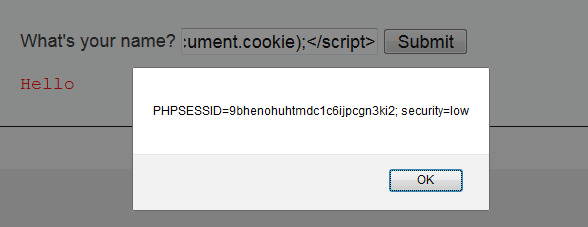
\includegraphics[width=0.5\textwidth]{oui/images/xss/xss5.PNG}
  \caption{Récupération du cookie utilisateur}
  \label{fig:courbe-tikz}
\end{figure}

On récupère bien le cookie de l'utilisateur avec qui on est connecté. On pourrait donc imaginer une attaque par le biais de cette faille: 


\begin{figure}[htp!]
  \centering
  \setlength\figureheight{7cm}
  \setlength\figurewidth{9cm}
  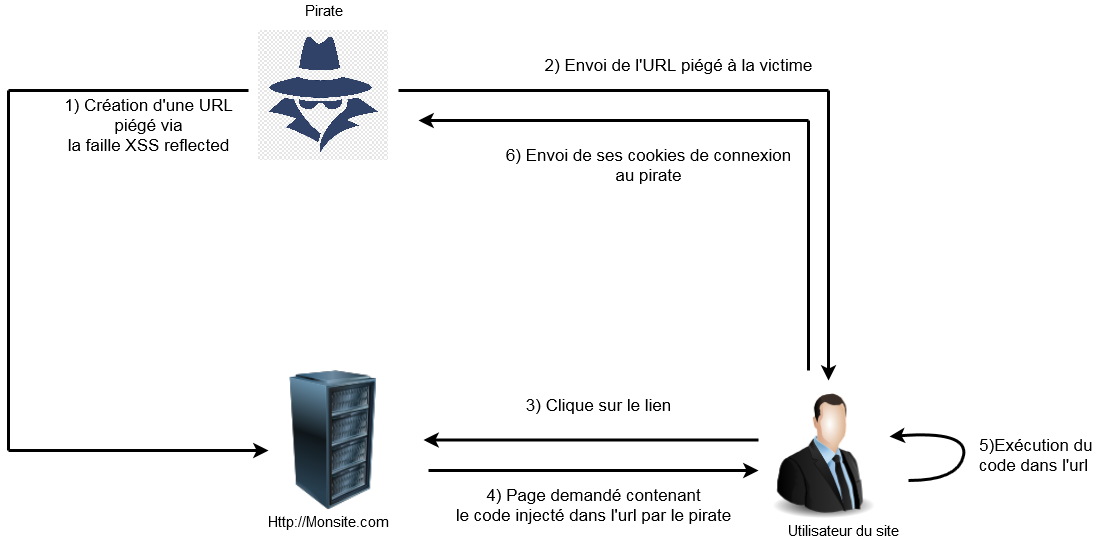
\includegraphics[width=0.75\textwidth]{oui/images/xss/Untitled Diagram(3).png}
  \caption{Attaque par vol de cookies}
  \label{fig:courbe-tikz}
\end{figure}

\newpage

\subsection{XSS Permanente}

Ce type de vulnérabilité se produit lorsque les données fournis par un utilisateur sont stockées sur un serveur (fichier, base de données...) afin d’être par la suite affichées à chaque ouverture du site. Nous pouvons prendre l’exemple des forums dans lesquels un utilisateur peut par exemple injecter un script qui sera visible par tous et donc provoquer des failles chez un grand nombre d’utilisateurs. On se rend rapidement compte que cette faille est véritablement dangereuse. Grâce à celle-ci, on peut par exemple récupérer les cookies des utilisateurs ou faire exécuter du code malveillant à notre insu. On peut également récupérer les cookies de tous les utilisateurs qui consultent la page contenant le code du pirate.

\subsection{Faille DOM based XSS}

DOM est l’abréviation de Document Object Model-based. 
Ce type d’attaque a lieu directement dans le navigateur de la victime sans passer par le serveur web. La page web ne change pas, en revanche le code côté client qui est contenu dans la page s'exécute de manière inopinée, et cela est engendré par les modifications malveillantes apportées à l’environnement DOM.
Cette attaque a lieu dans la grande majorité des cas dans les nouvelles applications web car une grande quantité de code javascript est exécutée dans le navigateur de l’utilisateur.

\subsection{Détection de la présence d’une faille XSS}

Afin de détecter la présence d’une faille XSS, on peut commencer par taper dans un formulaire (commentaire, moteur de recherche, chat…) le code suivant:\\
<b>Faille</b>\\
Si le message suivant est affiché: Aucun résultat trouvé pour le terme “Faille”, c’est qu’une faille XSS est présente.\\
Si le message suivant est affiché: Aucun résultat trouvé pour le terme <b>Faille</b>, cela signifie que le site est convenablement sécurisé.\\
A la suite de la première étape décrite ci-dessus, il est possible d’utiliser un script Javascript dans un champ de formulaire afin d’être convaincu de l’existence d’une faille XSS.
On peut par exemple avoir recours au script suivant:\\
<script > alert (Attention ce site est vulnérable face aux attaques XSS) </script >\\
Afin de savoir si le site web est vulnérable aux attaques XSS, il suffit donc de taper ce script dans un formulaire, si aucun message ne s’affiche, dans ce cas vous ne risquez pas de vous retrouver face à une faille XSS sur le site en question, en revanche si le message “Attention ce site est vulnérable face aux attaques XSS” s’affiche, dans ce cas là il est préférable pour vous de changer de site.

\subsection{Se protéger d'une faille XSS}

La solution permettant de se protéger face à une attaque XSS est de convertir les données. Pour ce qui est du langage PHP, il est courant d’avoir recours aux fonctions htmlentities() et htmlspecialchars() qui permettent de convertir les caractères spéciaux en entités HTML. De ce fait, les données ne seront plus interprétées par le navigateur, mais simplement affichées.\\

\noindent \textbf{Conclusion : }\\

La faille XSS est l’une des failles qu’on retrouve le plus couramment sur le web. Cela est expliqué par le fait que cette faille permet un grand nombre d’attaques. On peut par exemple grâce à cette faille détourner un formulaire afin de rediriger l’utilisateur vers un site malveillant. Cela permet en autres de voler les cookies d’un utilisateur et donc par la même occasion d’obtenir son login et son mot de passe.
Heureusement, cette faille peut être aisément évitée en prenant la peine de traiter correctement les données en entrée.

%\newpage


\section{Failles SQL}

Le SQL est un langage de programmation orienté vers les bases de données. Ces bases de données contiennent en général des identifiants et des mots de passe qu'il faut absolument sécuriser. Lors d'une connexion via formulaire sur une page Web, l'utilisateur doit remplir les champs libres qui seront ensuite comparés aux comptes dans la base de données. Les schéma ci-dessous peut faciliter la compréhension du fonctionnement d'authentification :

\begin{figure}[htp!]
  \centering
  \setlength\figureheight{7cm}
  \setlength\figurewidth{9cm}
  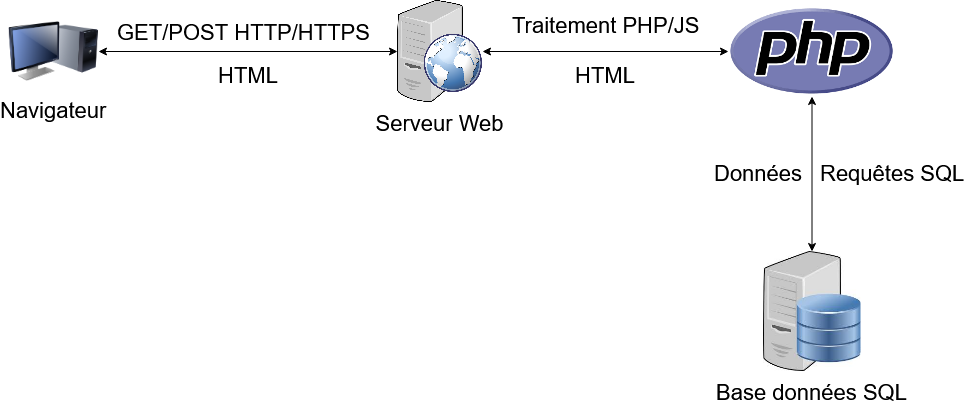
\includegraphics[width=0.8\textwidth]{oui/Ancien/imangeancien/SQLi/SQLDiagram.png}
  \caption{Fonctionnement d'un formulaire}
  \label{fig:courbe-tikz}
\end{figure}

Depuis un navigateur, nous allons donc remplir le formulaire de connexion qui va être envoyé vers le serveur Web qui contient un serveur PHP. Ce dernier va traiter le code PHP pour récupérer (le plus souvent en POST) et faire une requête SQL vers la base de données afin de vérifier que les données correspondent. Si c'est le cas, le serveur PHP laisse l'utilisateur entrer sur le site.\\
Voici la structure d'une base de données :

\begin{figure}[htp!]
  \centering
  \setlength\figureheight{7cm}
  \setlength\figurewidth{9cm}
  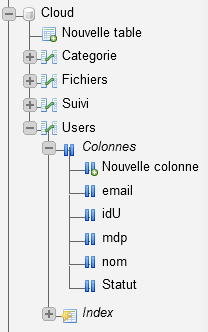
\includegraphics[width=0.3\textwidth]{oui/Ancien/imangeancien/SQLi/BD.PNG}
  \caption{Exemple d'une base de données}
  \label{fig:courbe-tikz}
\end{figure}

Dans cet exemple, la base de données se nomme "Cloud" et contient plusieurs tables : "Categories", "Fichiers", "Suivi" et "Users". Ensuite, chaque table contient des colonnes qui sont ici dans la table "Users": "email", "idU", "mdp", "nom", "Statut". On comprend donc que les données de chaque utilisateurs sont stockées dans la colonne Users. Le PHP va donc essayer de faire correspondre ce qui a été rentré dans le formulaire et ce qui est présent dans cette table afin de valider ou non la connexion.\\
Une injection SQL consiste à injecter du code SQL dans une requête SQL dans le but de la détourner et donc de modifier le résultat que cette requête était censé afficher. Cela permet également d’afficher du contenu qui était en toute logique dissimulé (table des users avec les identifiant et mot de passe qui vont avec). Enfin, une insertion SQL permet d’ajouter, de supprimer ou de modifier une base de données.

\subsection{Détection faille SQL}

Les failles SQL peuvent être exploitées via l’outil SQLMAP. Ce dernier va tenter d’injecter des SELECT dans la base de données et de nous fournir un résultat. Pour mieux comprendre le concept, nous pouvons essayer SQLMAP sur des sites spécialisés en test SQL. Sur celui-ci, nous pouvons tester au niveau de l’URL si une injection est possible :

\begin{figure}[htp!]
  \centering
  \setlength\figureheight{7cm}
  \setlength\figurewidth{9cm}
  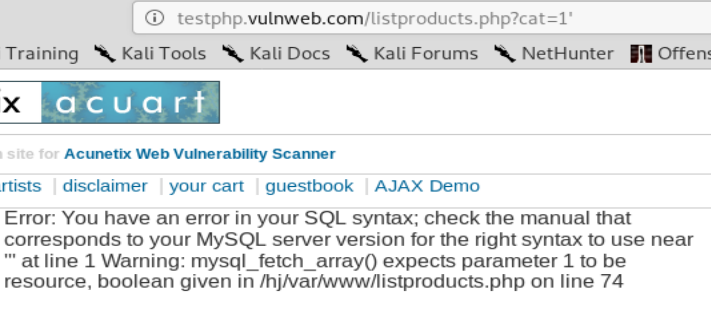
\includegraphics[width=0.8\textwidth]{oui/Ancien/imangeancien/SQLi/1.PNG}
  \caption{Détection d'une faille SQL}
  \label{fig:courbe-tikz}
\end{figure}

Comme on peut le voir, pour tester la sécurité de la base de données aux injections SQL, il nous a juste fallu ajouter, dans l'URL, une apostrophe après le GET du site web. Ainsi, la base de données nous envoie un message d’erreur. Cette erreur nous indique que les données tapées par les utilisateurs ne sont pas vérifiées du côté serveur.

\subsection{Exploitation faille SQL}
\subsubsection{SQLMAP}

Passons maintenant à l’outil SQLMAP en rentrant la commande suivante :

\begin{figure}[htp!]
  \centering
  \setlength\figureheight{7cm}
  \setlength\figurewidth{9cm}
  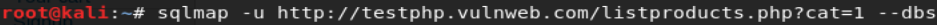
\includegraphics[width=0.9\textwidth]{oui/Ancien/imangeancien/SQLi/2.PNG}
  \caption{Commande SQLMAP}
  \label{fig:courbe-tikz}
\end{figure}

L’option “-u” va nous permettre d’entrer une URL et le “--dbs” va nous permettre d’afficher les bases de données. Le résultat nous est envoyé sous cette forme :

\begin{figure}[htp!]
  \centering
  \setlength\figureheight{7cm}
  \setlength\figurewidth{9cm}
  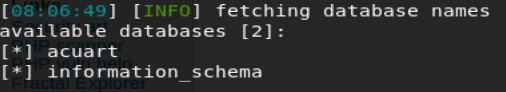
\includegraphics[width=0.8\textwidth]{oui/Ancien/imangeancien/SQLi/3.PNG}
  \caption{Résultat}
  \label{fig:courbe-tikz}
\end{figure}

Il existe alors deux bases de données qui sont acuart et information\_schema. Etant donné que notre site cible est Acuart, nous allons visualiser ses tables :

\begin{figure}[htp!]
  \centering
  \setlength\figureheight{7cm}
  \setlength\figurewidth{9cm}
  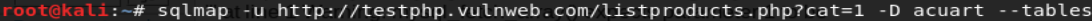
\includegraphics[width=0.9\textwidth]{oui/Ancien/imangeancien/SQLi/4.PNG}
  \caption{Commande pour visualiser les tables}
  \label{fig:courbe-tikz}
\end{figure}

\begin{figure}[htp!]
  \centering
  \setlength\figureheight{7cm}
  \setlength\figurewidth{9cm}
  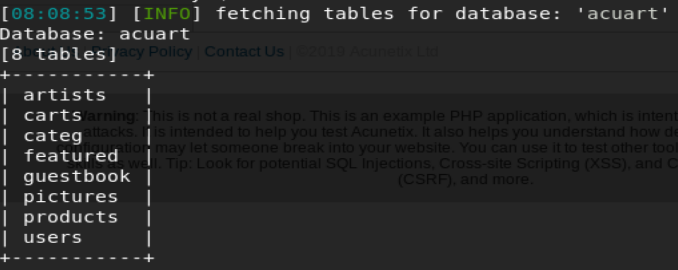
\includegraphics[width=0.8\textwidth]{oui/Ancien/imangeancien/SQLi/5.PNG}
  \caption{Résultat}
  \label{fig:courbe-tikz}
\end{figure}

A l’intérieur de la base de données, il existe une table users que nous allons dévoiler :

\begin{figure}[htp!]
  \centering
  \setlength\figureheight{7cm}
  \setlength\figurewidth{9cm}
  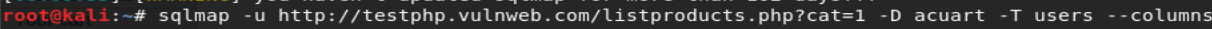
\includegraphics[width=0.9\textwidth]{oui/Ancien/imangeancien/SQLi/6.PNG}
  \caption{Commande pour visualiser les colonnes}
  \label{fig:courbe-tikz}
\end{figure}

\begin{figure}[htp!]
  \centering
  \setlength\figureheight{7cm}
  \setlength\figurewidth{9cm}
  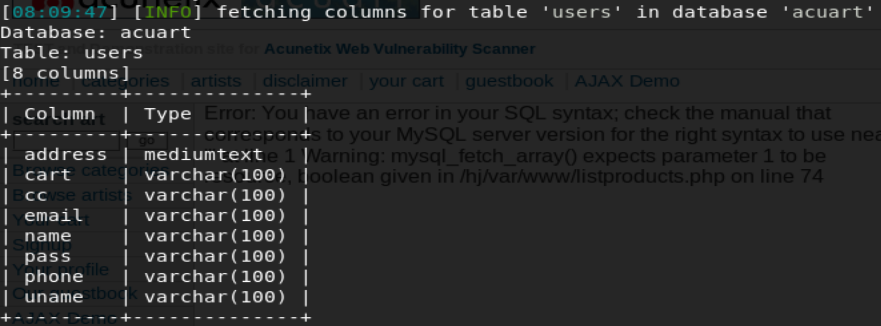
\includegraphics[width=0.8\textwidth]{oui/Ancien/imangeancien/SQLi/7.PNG}
  \caption{Résultat}
  \label{fig:courbe-tikz}
\end{figure}

Dans notre cas, les seules informations dont nous avons besoin sont : name, pass et uname :

\begin{figure}[htp!]
  \centering
  \setlength\figureheight{7cm}
  \setlength\figurewidth{9cm}
  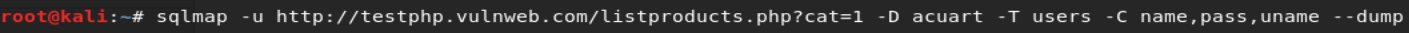
\includegraphics[width=0.9\textwidth]{oui/Ancien/imangeancien/SQLi/8.PNG}
  \caption{Commande pour visualiser un SELECT}
  \label{fig:courbe-tikz}
\end{figure}

\begin{figure}[htp!]
  \centering
  \setlength\figureheight{7cm}
  \setlength\figurewidth{9cm}
  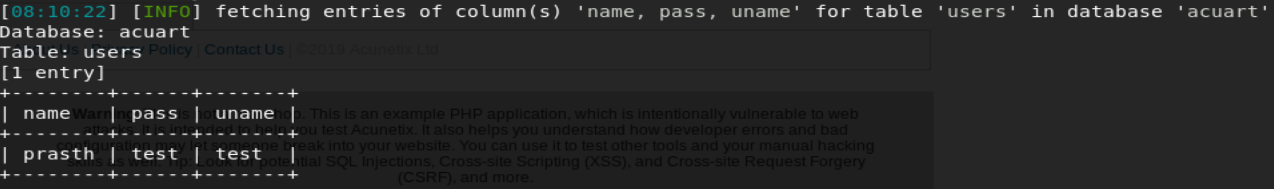
\includegraphics[width=0.9\textwidth]{oui/Ancien/imangeancien/SQLi/9.PNG}
  \caption{Résultat}
  \label{fig:courbe-tikz}
\end{figure}

\vspace{4cm}

Il existe donc un utilisateur test que nous allons essayer pour nous connecter :

\begin{figure}[htp!]
  \centering
  \setlength\figureheight{7cm}
  \setlength\figurewidth{9cm}
  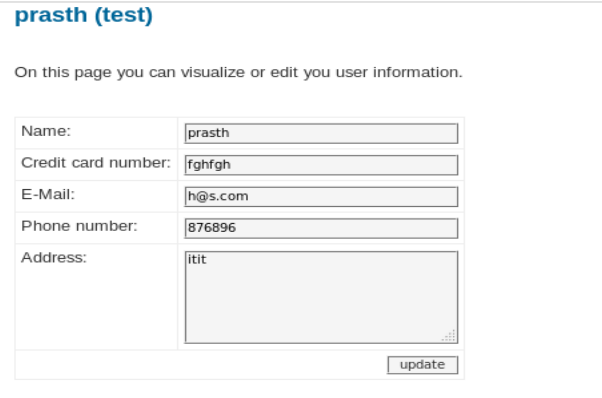
\includegraphics[width=0.6\textwidth]{oui/Ancien/imangeancien/SQLi/11.PNG}
  \caption{Connexion}
  \label{fig:courbe-tikz}
\end{figure}

Nous avons réussi à nous connecter via une faille SQL.

\subsubsection{SQLi}
Cependant, nous aurions pu éviter de passer par SQLMAP. En effet, si nous avions voulu juste rentrer dans un site exploitable, nous aurions juste pu injecter nous-même une condition. Pour cela, nous allons nous rendre sur un site créé par l’IUT de Blagnac proposant un CTF en ligne. Nous allons donc aller dans la partie SQLi pour essayer une injection visible en \textbf{figure \ref{fig:sqli}}.

\begin{figure}[htp!]
  \centering
  \setlength\figureheight{7cm}
  \setlength\figurewidth{9cm}
  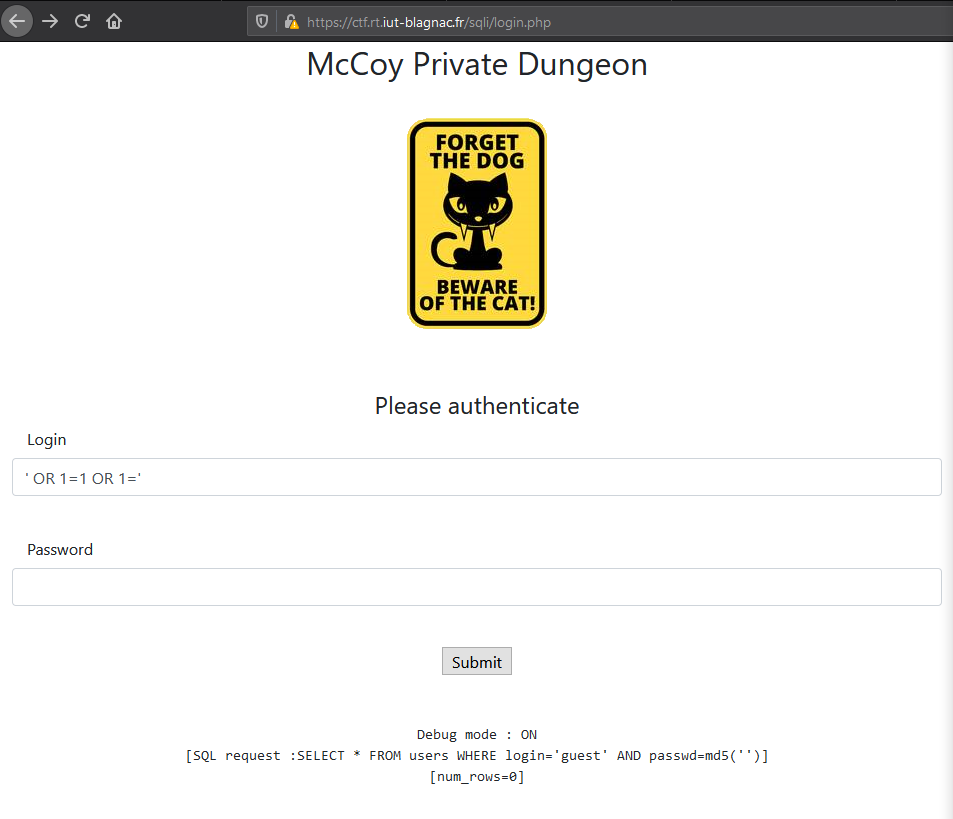
\includegraphics[width=0.7\textwidth]{oui/Ancien/imangeancien/SQLi/12.PNG}
  \caption{SQLi}
  \label{fig:sqli}
\end{figure}

Cette injection va nous permettre d’ajouter une condition dans la requête qui sera toujours vraie car 1 sera toujours égal à 1. On pourra alors se connecter et entrer dans le site comme on peut le voir sur la \textbf{figure \ref{fig:sqlicon}}.

\begin{figure}[htp!]
  \centering
  \setlength\figureheight{7cm}
  \setlength\figurewidth{9cm}
  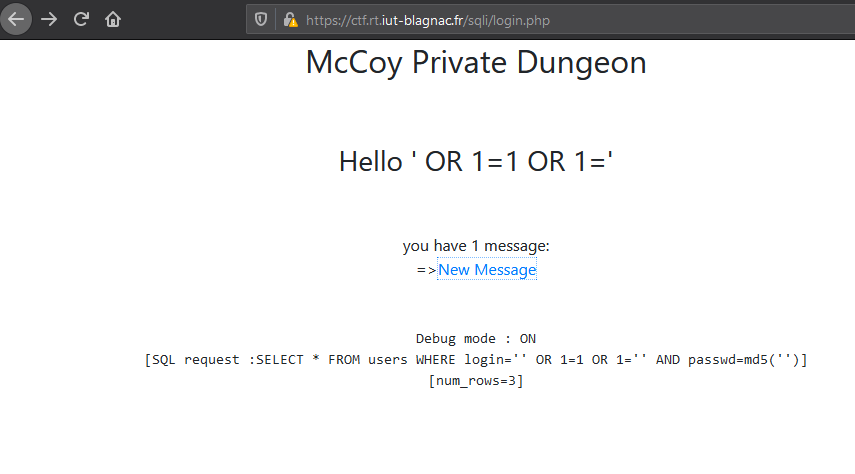
\includegraphics[width=0.7\textwidth]{oui/Ancien/imangeancien/SQLi/13.PNG}
  \caption{Connexion}
  \label{fig:sqlicon}
\end{figure}

\newpage
\subsection{Protection faille SQL}

Bien entendu, le mot d’ordre est vigilance. Il est utile pour tout administrateur de vérifier constamment les données entrées par l’utilisateur. Les paramètres d’URL et les formulaires (connexion, recherche) sont des potentiels risques d’attaque par injection.
Grâce au langage PHP, il est maintenant possible d’avoir recours à des librairies qui auront le rôle de préparer des requêtes SQL avant leurs exécutions. Ces librairies permettent entres autres de valider les données des requêtes.
PDO est la plus connue de ces librairies. Cette fonction est directement inclue dans la classe MySQLi pour les nouvelles versions de PHP.
Il est utile de camoufler les messages d’erreurs qui peuvent s’afficher sur votre site (comme avec l’exemple de l’apostrophe dans l’URL ci-dessus) dans la mesure où ces messages permettent aux hackers d’avoir des informations sur votre base de données. 
Afin d’éviter les caractères spéciaux, il est pratique d’utiliser la fonction :\\ mysqli\_real\_escape\_string()\\
Enfin, il est préférable d’utiliser des comptes utilisateurs qui ont des droits limités. Cela permet d’empêcher l'éventuel hacker de modifier ou supprimer des éléments de la base de données.\\

\noindent \textbf{Conclusion}

Environ un site sur cinq est vulnérable aux injections SQL. Cela est dû au fait qu’une simple erreur peut compromettre la sécurité de la base, des utilisateurs et même du serveur. Pour cette raison, c’est l’une des failles les plus dangereuses pour les applications ayant recours à une base de données. Plus inquiétant encore, les injections SQL sont en augmentation depuis qu'il existe des programmes d'injections SQL automatisés, qui permettent aux hackers de prendre possession d’encore plus de données que par le passé. Heureusement, de simples techniques permettent se protéger de ce type de faille.







\newpage
\section{Failles par Proxy}

Un proxy est un élément du réseau fonctionnant au niveau de la couche 7 (application) du modèle OSI. Un proxy peut être considéré comme un intermédiaire entre deux personnes surtout quand celles-ci ne parlent pas le même langage. Cela signifie qu'un proxy va intercepter toutes les requêtes entre un serveur et un client. Nous allons dans cette partie exploiter ce concept afin d'exploiter les failles d'un formulaire et contourner des sécurités via l'outil Burpsuite.

\subsection{Burpsuite}

\subsubsection{Définition}

Burpsuite est un logiciel complet permettant d’effectuer des tests d’intrusion ou de vulnérabilités (XSS, CSRF) sur des applications Web. Cet outil peut s’utiliser comme un proxy Web dans le but de chercher  et capturer toutes les requêtes Web des utilisateurs au sein d’un LAN. Ce dernier inclut notamment des procédés automatiques dans le but de travailler plus rapidement et plus efficacement.\\
Nous allons donc voir son fonctionnement.

\subsubsection{Fonctionnement}

Burpsuite se présente sous la forme d’une interface graphique:

\begin{figure}[htp!]
  \centering
  \setlength\figureheight{7cm}
  \setlength\figurewidth{9cm}
  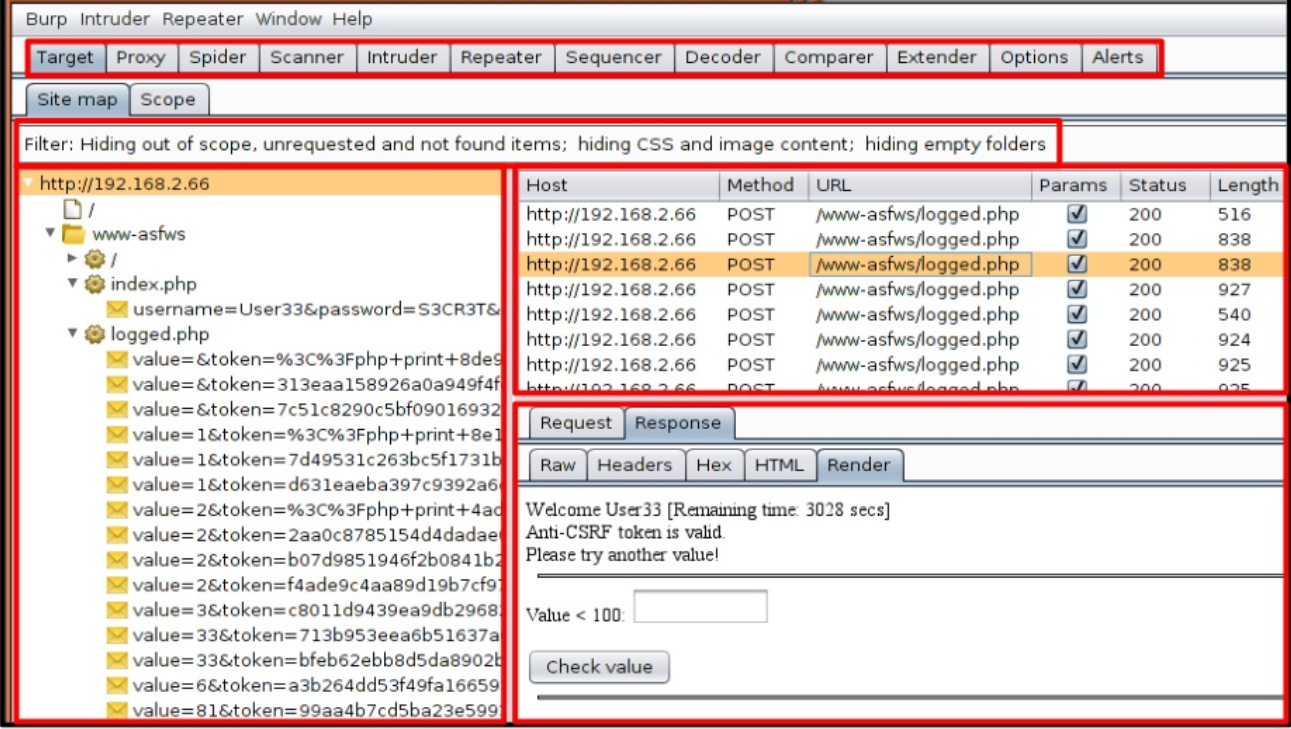
\includegraphics[width=0.6\textwidth]{oui/Ancien/imangeancien/burpsuite/burpsuite1.PNG}
  \caption{Interface graphique}
  \label{fig:courbe-tikz}
\end{figure}

\noindent Nous avons 3 types d’outils dans Burpsuite:\\

\noindent Les outils centraux:\\
- \textbf{Proxy} : Permet de configurer un proxy dans le but d’intercepter des requêtes web ou de les modifier avant de les transmettre au serveur web.\\
- \textbf{Site map} : Permet d’avoir une vue arborescente du trafic observé.\\


\noindent Les outils manuels:\\
- \textbf{Intruder}: Émission en masse de requêtes HTTP/HTTPS.\\
- \textbf{Repeater}: Permet la modification avant l’envoi de nos requêtes.\\

\noindent Les outils automatiques:\\
- \textbf{Spider}: Cet outil permet la récolte d’informations passives comme la détection de ressources et la collecte active.\\
- \textbf{Scanner}: Il va rechercher automatiquement des vulnérabilités (via le mode passif ou actif).\\

\noindent Les autres outils:\\
- \textbf{Sequencer}: Permet de  tester l'existence aléatoire des sessions avec jetons (token).\\
- \textbf{Decoder}: Conversion URL/HTML/Base64/Hexa/Octal/Binaire/GZip + hashes.\\

Burpsuite permet également la configuration de macros dans le but d’automatiser des tâches. De plus, l’avantage de Burpsuite réside dans la possibilité d’une configuration multiple, mais également, dans ses nombreuses fonctionnalités permettant d’aider les pentesteurs les plus expérimentés.\\

Ainsi, dans le cas d’un audit de sécurité ou d’un CTF, nous pouvons utiliser cet outil pour capturer le trafic des utilisateurs et ainsi récupérer des mots de passe ou des cookies de connexions pour se connecter à des sites (Gmail, Facebook,...).\\

\subsubsection{Exemple d’utilisation sur un CTF:}

\noindent Dans le cas où nous avons un formulaire de connexion, nous pouvons utiliser le mode Intercept de Burpsuite pour tester la sécurité de ce dernier, et ainsi injecter ou non du code malveillant comme le montre ce schéma :

\begin{figure}[htp!]
  \centering
  \setlength\figureheight{7cm}
  \setlength\figurewidth{9cm}
  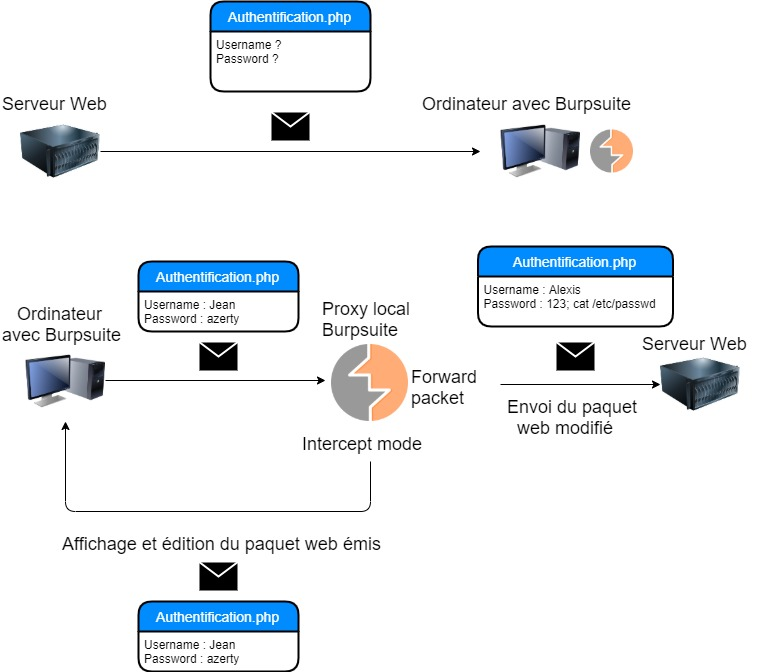
\includegraphics[width=1\textwidth]{oui/Ancien/imangeancien/burpsuite/Burpsuite-Fonctionnement.jpg}
  \caption{Fonctionnement du mode Intercept de Burpsuite}
  \label{fig:courbe-tikz}
\end{figure}

\newpage
\noindent Pour cela, il faut aller dans la catégorie proxy et choisir l’adresse IP du proxy à utiliser:

\begin{figure}[htp!]
  \centering
  \setlength\figureheight{7cm}
  \setlength\figurewidth{9cm}
  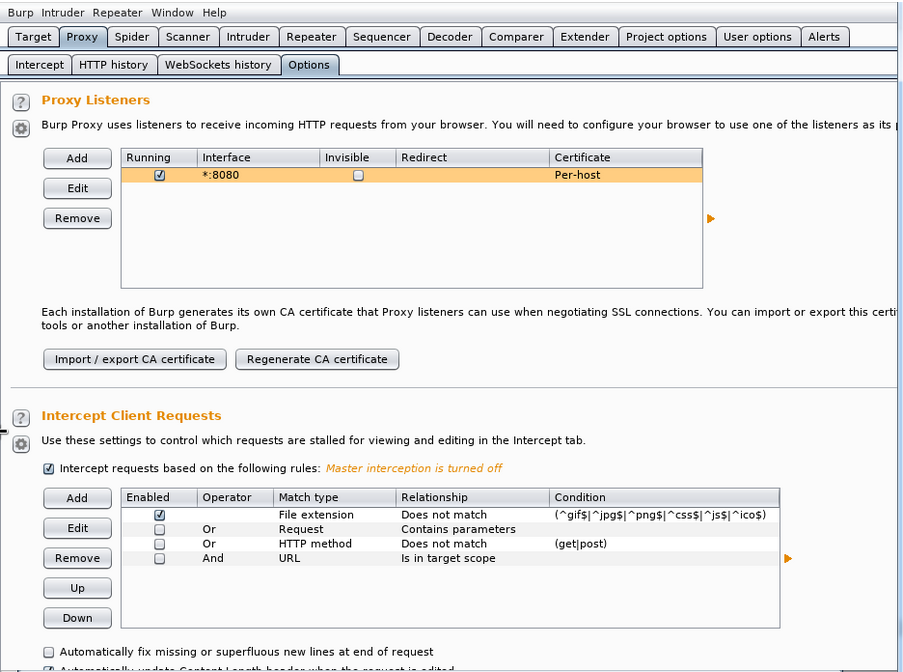
\includegraphics[width=0.8\textwidth]{oui/Ancien/imangeancien/burpsuite/burpsuite2.PNG}
  \caption{Mise en place du proxy BurpSuite}
  \label{fig:courbe-tikz}
\end{figure}
Dans notre cas, nous prendrons toutes les adresses IP de notre interface web (d’où le “*”) sur le port 8080. Ensuite, sur un ordinateur client, il suffit de préciser dans le navigateur le proxy à utiliser:
\begin{figure}[htp!]
  \centering
  \setlength\figureheight{7cm}
  \setlength\figurewidth{9cm}
  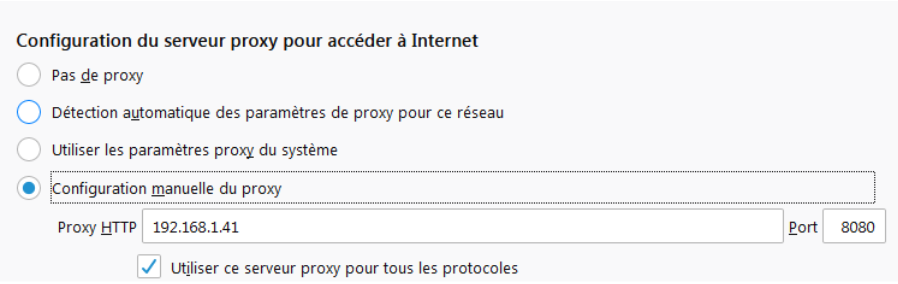
\includegraphics[width=0.8\textwidth]{oui/Ancien/imangeancien/burpsuite/burpsuite3.PNG}
  \caption{Mise en place du proxy coté client}
  \label{fig:courbe-tikz}
\end{figure}\\
On peut donc commencer les tests. Il faudra mettre Burpsuite sur le mode “intercept on” pour intercepter toutes les requêtes.\\

\newpage
\noindent Prenons le cas de ce formulaire en HTTP :
\begin{figure}[htp!]
  \centering
  \setlength\figureheight{7cm}
  \setlength\figurewidth{9cm}
  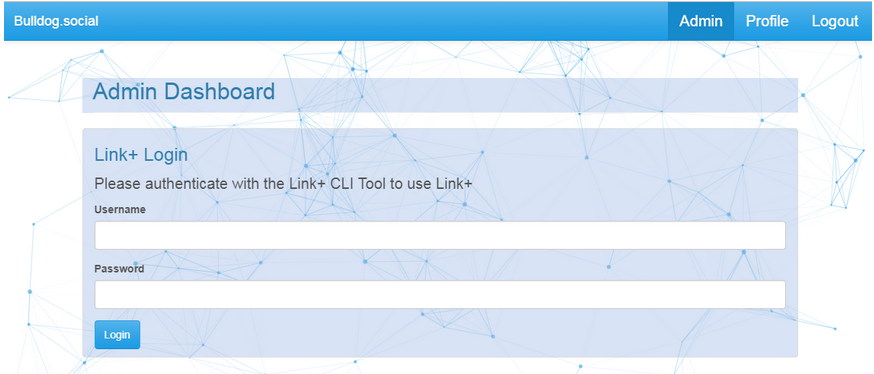
\includegraphics[width=1\textwidth]{oui/Ancien/imangeancien/burpsuite/burpsuite4.PNG}
  \caption{Formulaire Web}
  \label{fig:courbe-tikz}
\end{figure}\\
\noindent Par exemple, nous allons entrer un username et un password :
\begin{figure}[htp!]
  \centering
  \setlength\figureheight{7cm}
  \setlength\figurewidth{9cm}
  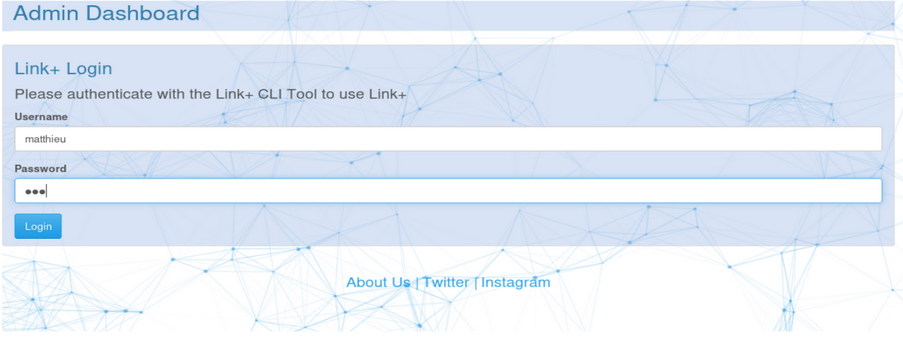
\includegraphics[width=1\textwidth]{oui/Ancien/imangeancien/burpsuite/burpsuite5.PNG}
  \caption{Formulaire Web}
  \label{fig:courbe-tikz}
\end{figure}\\
Comme nous pouvons le voir sur Burpsuite, on récupère la requête envoyée au serveur :
\newpage
\begin{figure}[htp!]
  \centering
  \setlength\figureheight{7cm}
  \setlength\figurewidth{9cm}
  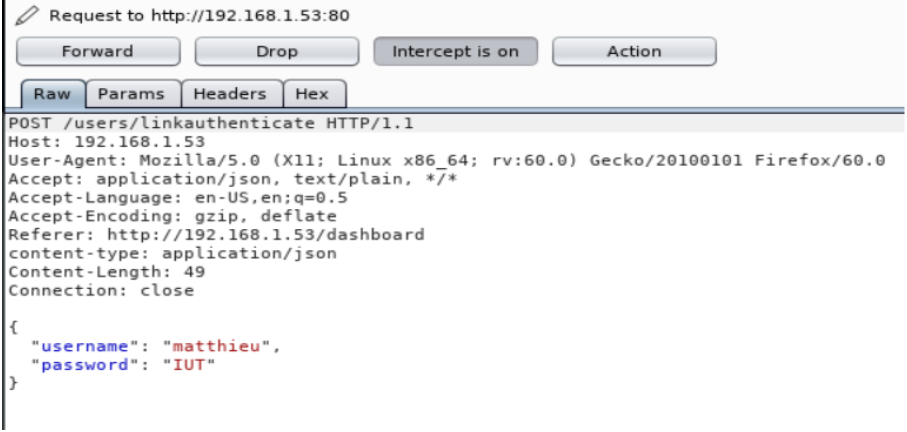
\includegraphics[width=1\textwidth]{oui/Ancien/imangeancien/burpsuite/burpsuite6.PNG}
  \caption{Interception requête HTTP}
  \label{fig:courbe-tikz}
\end{figure}

\noindent On peut alors la modifier avant de la transmettre au serveur :
\begin{figure}[htp!]
  \centering
  \setlength\figureheight{7cm}
  \setlength\figurewidth{9cm}
  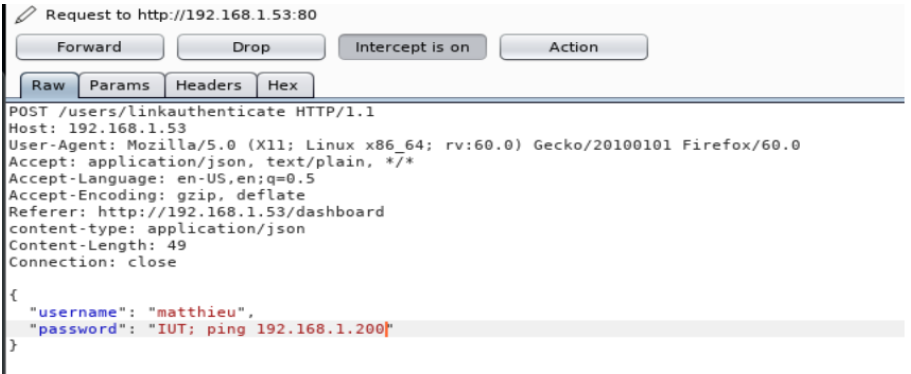
\includegraphics[width=1\textwidth]{oui/Ancien/imangeancien/burpsuite/burpsuite7.PNG}
  \caption{Modification de la requête}
  \label{fig:courbe-tikz}
\end{figure}\\
Dans notre cas, nous allons essayer d’injecter la commande "ping" pour tester la sécurité du champ “password”.\\

\newpage

\noindent Si on scrute le réseau avec Wireshark:
\begin{figure}[htp!]
  \centering
  \setlength\figureheight{7cm}
  \setlength\figurewidth{9cm}
  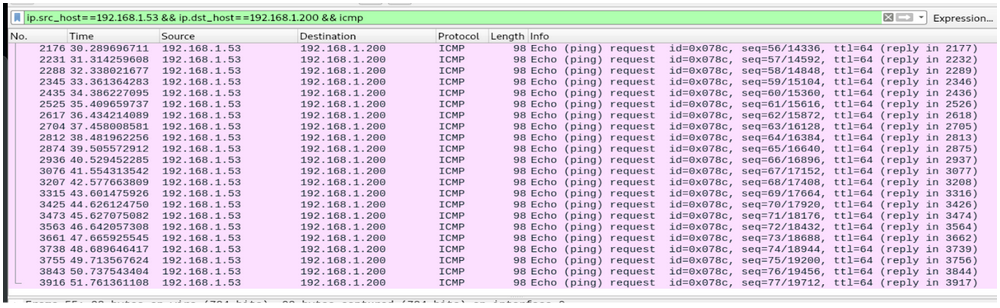
\includegraphics[width=1\textwidth]{oui/Ancien/imangeancien/burpsuite/burpsuite8.PNG}
  \caption{Modification de la requête}
  \label{fig:courbe-tikz}
\end{figure}

Le ping fonctionne bien. Cela veut dire que l'on peut injecter n’importe quelle commande dans le champ password. On pourrait par exemple injecter un reverse shell pour prendre le contrôle à distance la machine.

%\newpage

\section{Metasploit Framework}
\begin{figure}[htp!]
  \centering
  \setlength\figureheight{7cm}
  \setlength\figurewidth{9cm}
  
\includegraphics[width=0.2\textwidth]{oui/Ancien/imangeancien/metasploit.png}
  \caption{Logo de Metasploit}
  \label{fig:courbe-tikz}
\end{figure}

\subsection{Présentation de Metasploit}
Metasploit Pen Testing tool est un projet Open Source (sous Licence BSD modifiée) destiné à la sécurité informatique. Le but de ce projet est de rechercher des vulnérabilités ou des informations sur des systèmes automatisés de données ainsi que d'aider à la pénétration et au développement de signatures pour les IDS.\\

L'outil que nous allons étudier ici est "Metasploit Framework" qui est un sous projet de
Metasploit Pen Testing tool. C'est le sous projet le plus connu car il permet le développement et l’exécution d’exploits (logiciels permettant d’exploiter à son profit une vulnérabilité) contre une machine distante.\\

A la base, cet outil a été écrit en Perl. A la suite de quelques mises à jours, l'outil a complètement été réécrit en Ruby. Cet outil a été conçu par HD Moore en 2003 et il est désormais maintenu par la société Rapid7. C'est un outil très puissant permettant à des chercheurs en sécurité de travailler sur des potentielles vulnérabilités. Cependant, comme la plupart des outils de sécurité informatique, Metasploit peut être utilisé à la fois de manière légale et à la fois pour des activités illégales.\\
Aujourd'hui, le projet metasploit est hébergé sur le github de la société Rapid7, ce qui permet à des utilisateurs indépendants d'y développer des modules d'exploitation pour des vulnérabilités logicielles et de les poster dans le projet Git. Ainsi, chaque utilisateur peut contribuer au développement de cet outil. Cependant, avant chaque publication, la société Rapid7 teste et vérifie le bon fonctionnement de l'exploit avant de le mettre à disposition sur github.\\
Comme nous l’avons dit précédemment, Metasploit possède un Framework ce qui facilite le travail des contributeurs puisqu’ils peuvent utiliser des fonctions de ce dernier pour développer leurs exploits. Enfin, ce qui fait la “force” de Metasploit est qu’il peut regrouper beaucoup d’outils très intéressants tels que Nmap, Hydra ou encore John the ripper, le tout dans une seule console. Cela permet de centraliser beaucoup d’outils de Kali linux.
\subsection{Architecture modulaire}
\begin{figure}[htp!]
  \centering
  \setlength\figureheight{7cm}
  \setlength\figurewidth{9cm}
  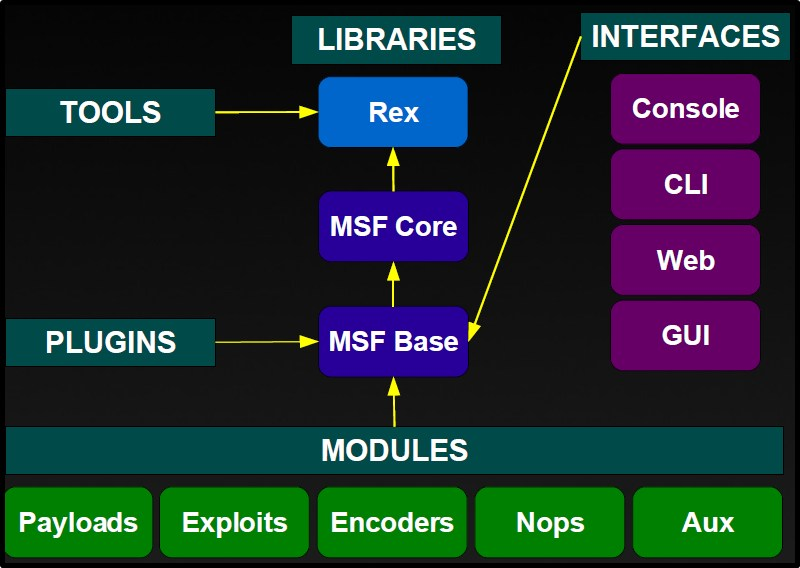
\includegraphics[width=0.5\textwidth]{oui/Ancien/imangeancien/Metasploit_Architecture.jpg}
  \caption{Architecture modulaire}
  \label{fig:courbe-tikz}
\end{figure}

La particularité de Metasploit est qu’il possède une architecture modulaire, ce qui permet un développement plus facile, une amélioration progressive du programme. De plus, les modules peuvent être rechargés sans redémarrage de l’application, ce qui est très pratique pour le développement.\\
Comme nous pouvons le constater sur ce schéma, il y 3 grandes parties qui composent Metasploit. La première est la librairie. Cette dernière permet de regrouper un grand nombre de fonctions et de programmes dans le but de constituer une API. Ainsi, lors de l’écriture d’un exploit ou d’un payload, le développeur n’aura qu'à connaître l’API de Metasploit pour son développement.\\
\noindent Metasploit utilise un système de librairie pour stocker ses fichiers.
\noindent La librairie est composée de :\\
- \textbf{Rex} – C’est la librairie principale regroupant la gestion des sockets, protocoles, encodeurs, SSL, SMB, HTTP, XOR, Base64, Unicode.\\
- \textbf{MSF::Core} – Cela permet de fournir l’API basique.\\
- \textbf{MSF::Base} Fournit l'API " amicale "et il fournit des API simplifiées à utiliser dans le framework.\\

\noindent Metasploit peut s’utiliser sur plusieurs interfaces:\\
- \textbf{Msfconsole} : Permet d’avoir une console Metasploit au sein d’un shell, elle est considérée comme l’interface la plus puissante et la plus complète.\\
- \textbf{MsfCli :} Permet d’utiliser Metasploit en ligne de commande ce qui peut être très pratique pour l’intégrer dans un script.\\
- \textbf{Msfweb:} Permet d’accéder à l’ensemble des outils de Metasploit sur une interface web. Facile d’utilisation.\\
- \textbf{Armitage:} Interface GUI de Metasploit. Cet outil est développé par Raphel Mudge et il regroupe tous les outils de Metasploit sous forme d’interface graphique. De plus, il supporte msfcli ainsi que msfconsole.\\

\noindent L’architecture de Metasploit peut également être représentée en modèle objet : 
\begin{figure}[htp!]
  \centering
  \setlength\figureheight{7cm}
  \setlength\figurewidth{9cm}
  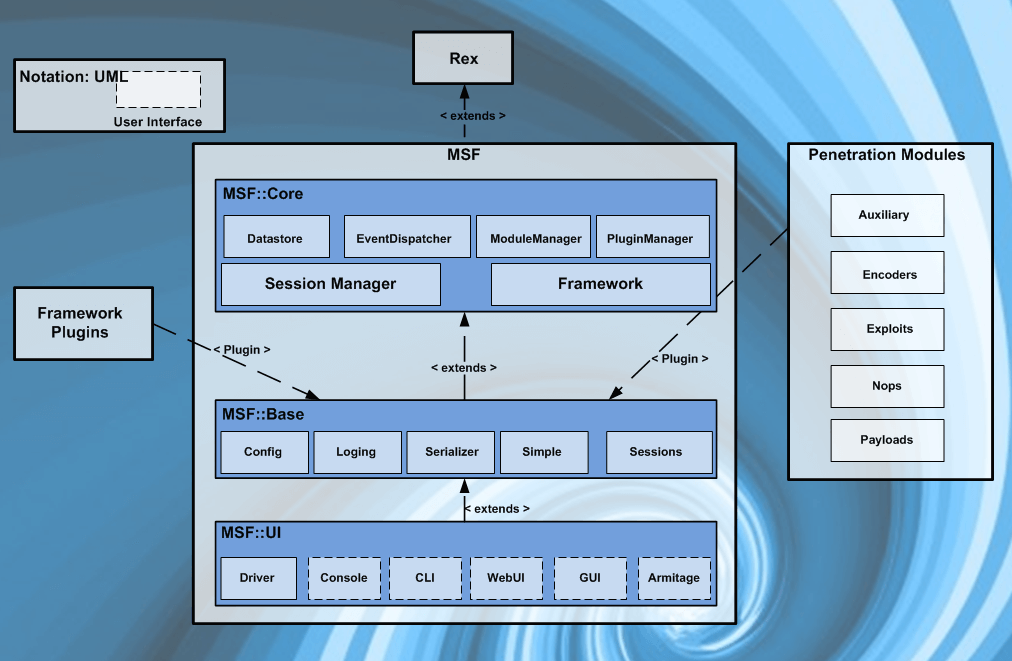
\includegraphics[width=0.8\textwidth]{oui/Ancien/imangeancien/msfarch2.png}
  \caption{Architecture modèle objet}
  \label{fig:courbe-tikz}
\end{figure}\\
Tous les modules de Metasploits sont des classes Ruby. On peut donc en déduire d'une part que d'après ce schéma, la classe Modules hérite d'une classe spécifique. Cette classe spécifique hérite de la classe Msf::Module et enfin, tous les modules se partagent une API commune.\\

D'autres part, on peut accéder aux modules depuis le terminal avec la commande suivante:
\begin{figure}[htp!]
  \centering
  \setlength\figureheight{7cm}
  \setlength\figurewidth{9cm}
  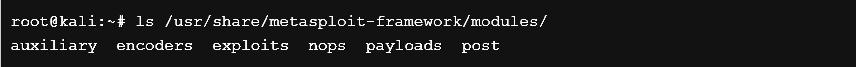
\includegraphics[width=1\textwidth]{oui/Ancien/imangeancien/modules.PNG}
  \caption{Accès aux modules de Metasploit}
  \label{fig:courbe-tikz}
\end{figure}

\subsection{Base de données de Metasploit}
\noindent Le Framework Metasploit fournit un support des bases de données utilisant  PostgreSQL. Cette dernière stocke des informations, telles que les données de l'hôte, les résultats de scans comme nmap et les résultats d'exploitation. Cela peut être très utile si on fait beaucoup d'exploits ou de tests d'intrusions sur des machines.

\noindent Cependant, cette base de données n'a pas besoin d'être lancée pour exécuter Metasploit mais elle est très utile pour stocker des logs de scan ou d'exploit.\\

\noindent Pour lancer PostgreSQL sous Kali linux, on utilise la commande suivante:
\begin{figure}[htp!]
  \centering
  \setlength\figureheight{7cm}
  \setlength\figurewidth{9cm}
  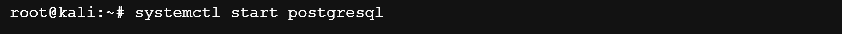
\includegraphics[width=1\textwidth]{oui/Ancien/imangeancien/metasploit/db_launch.PNG}
  \caption{Lancement du service PostgreSQL}
  \label{fig:courbe-tikz}
\end{figure}

\noindent On peut si on le souhaite, créer une base de données en local pour Metasploit. Pour initialiser une base de données, on utilise la commande suivante:

\begin{figure}[htp!]
  \centering
  \setlength\figureheight{7cm}
  \setlength\figurewidth{9cm}
  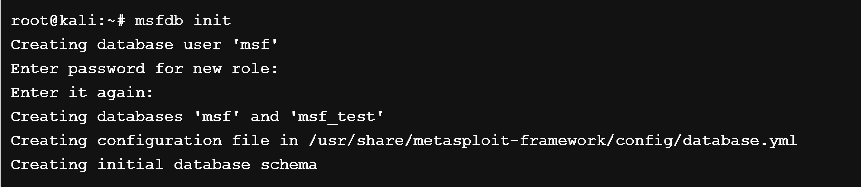
\includegraphics[width=0.8\textwidth]{oui/Ancien/imangeancien/metasploit/db_init.PNG}
  \caption{Création de la base de données}
  \label{fig:courbe-tikz}
\end{figure}

Ainsi, cette commande va créer plusieurs utilisateurs avec des mots de passes et créer deux bases de données : msf et msf\_test. On peut également vérifier la configuration de notre base données qui se trouve dans le fichier \textbf{/usr/share/metasploit-framework/config/ \\ database.yml}:

%\newpage

\begin{figure}[htp!]
  \centering
  \setlength\figureheight{7cm}
  \setlength\figurewidth{9cm}
  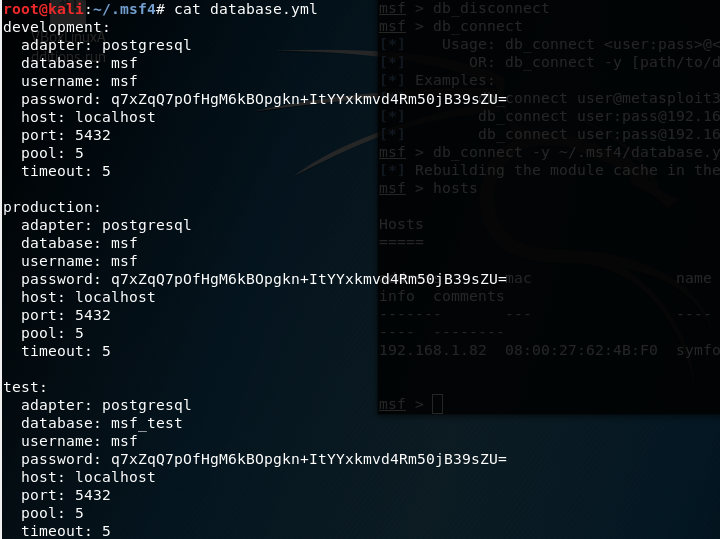
\includegraphics[width=0.8\textwidth]{oui/Ancien/imangeancien/metasploit/database.PNG}
  \caption{Fichier database.yml}
  \label{fig:courbe-tikz}
\end{figure}


\noindent On peut voir que la base de données a bien été lancée :

\begin{figure}[htp!]
  \centering
  \setlength\figureheight{7cm}
  \setlength\figurewidth{9cm}
  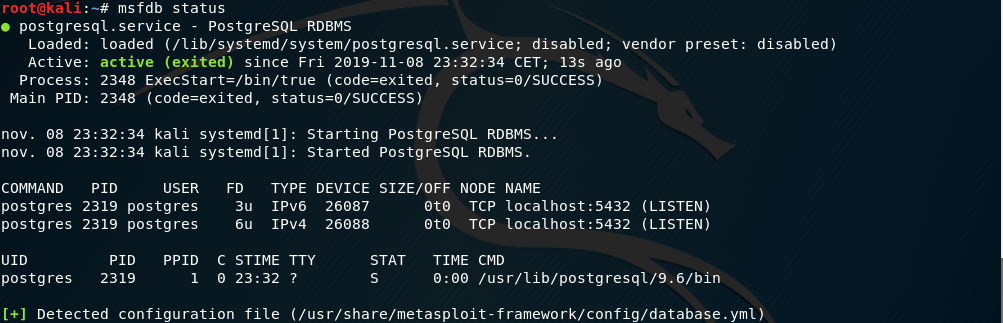
\includegraphics[width=0.8\textwidth]{oui/Ancien/imangeancien/metasploit/db_status1.PNG}
  \caption{Status de la DB}
  \label{fig:courbe-tikz}
\end{figure}

\noindent On peut voir qu'il y a 1'utilisateur qui a été créé msf" ainsi que 3 catégories "development" , "production" et "test". Ce fichier permet de récupérer les informations de connexion pour se connecter à la base de données.\\

\noindent En lançant Metasploit, on peut utiliser la commande \textbf{db\_connect} pour se connecter à notre base de données :

\begin{figure}[htp!]
  \centering
  \setlength\figureheight{7cm}
  \setlength\figurewidth{9cm}
  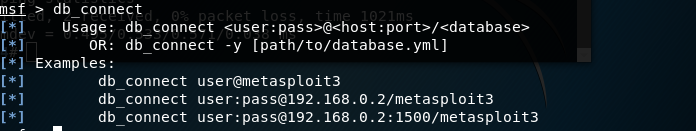
\includegraphics[width=0.8\textwidth]{oui/Ancien/imangeancien/metasploit/db_connect.PNG}
  \caption{Connexion à la base de données}
  \label{fig:courbe-tikz}
\end{figure}
\noindent Cette commande nous indique que nous pouvons nous connecter soit en rentrant directement l'utilisateur, le mot de passe, l'adresse IP et la base de données, soit en renseignant un fichier de connexion à utiliser comme le fichier \textbf{database.yml}.\\

\noindent Nous allons par exemple renseigner la méthode avec le fichier :

\begin{figure}[htp!]
  \centering
  \setlength\figureheight{7cm}
  \setlength\figurewidth{9cm}
  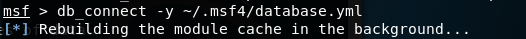
\includegraphics[width=0.8\textwidth]{oui/Ancien/imangeancien/metasploit/db_connect2.PNG}
  \caption{Connexion avec un fichier}
  \label{fig:courbe-tikz}
\end{figure}

\noindent On vérifie qu'on est bien connecté à la base de données :

\begin{figure}[htp!]
  \centering
  \setlength\figureheight{7cm}
  \setlength\figurewidth{9cm}
  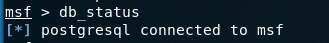
\includegraphics[width=0.5\textwidth]{oui/Ancien/imangeancien/metasploit/db_status2.PNG}
  \caption{Vérification de la connexion avec la DB}
  \label{fig:courbe-tikz}
\end{figure}

Une fois connecté à la base de données, on peut réaliser quelques actions intéressantes. Par exemple, on peut stocker le résultat d'un scan \textbf{nmap} avec la commande \textbf{db\_nmap} :

\begin{figure}[htp!]
  \centering
  \setlength\figureheight{7cm}
  \setlength\figurewidth{9cm}
  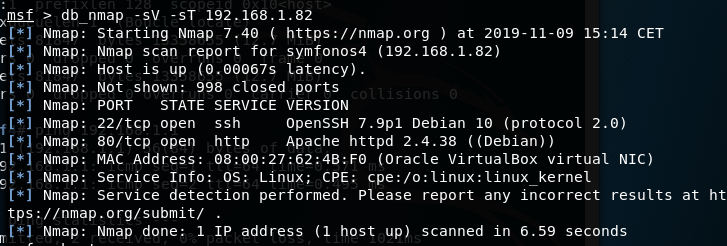
\includegraphics[width=0.8\textwidth]{oui/Ancien/imangeancien/metasploit/db_nmap.PNG}
  \caption{Scan NMAP avec DB}
  \label{fig:courbe-tikz}
\end{figure}

Pour l'exemple, on scanne une machine virtuelle de notre réseau local dans laquelle il y a des services ouverts potentiellement vulnérables.\\

La commande \textbf{hosts} permet de voir quelles sont les machines que nous avons scannées et qui sont stockées dans la base de données comme indiqué sur la \textbf{figure \ref{fig:meta-hote}}\\

\begin{figure}[h]
  \centering
  \setlength\figureheight{7cm}
  \setlength\figurewidth{9cm}
  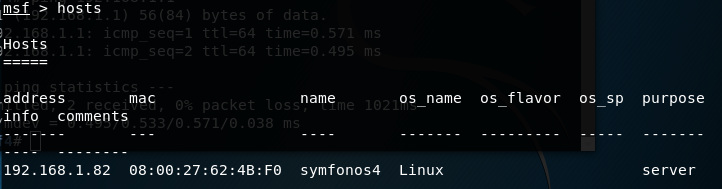
\includegraphics[width=0.8\textwidth]{oui/Ancien/imangeancien/metasploit/db_hosts.PNG}
  \caption{Hôtes scannés}
  \label{fig:meta-hote}
\end{figure}

La commande \textbf{services} permet de voir tous les services scannés avec nmap voir \textbf{figure \ref{fig:services-scan}}\\

\begin{figure}[h]
  \centering
  \setlength\figureheight{7cm}
  \setlength\figurewidth{9cm}
  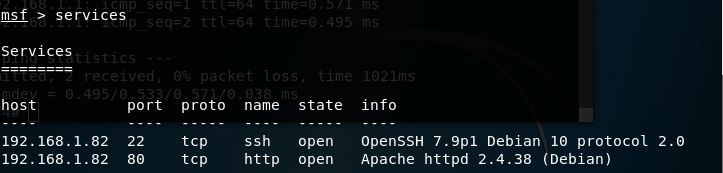
\includegraphics[width=0.8\textwidth]{oui/Ancien/imangeancien/metasploit/db_services.PNG}
  \caption{Services scannés}
  \label{fig:services-scan}
\end{figure}

Il est également possible de pouvoir exporter notre base de données en format .xml avec la commande suivante indiqué dans la \textbf{figure \ref{fig:xml-db}}
\begin{figure}[h]
  \centering
  \setlength\figureheight{7cm}
  \setlength\figurewidth{9cm}
  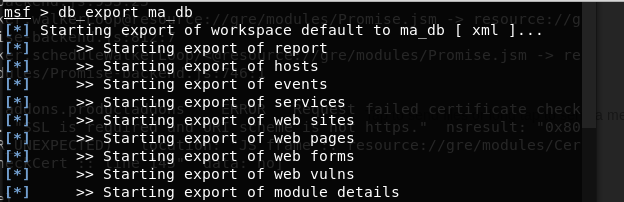
\includegraphics[width=0.8\textwidth]{oui/Ancien/imangeancien/metasploit/db_export.PNG}
  \caption{Exportation de la DB}
  \label{fig:xml-db}
\end{figure}

%\newpage

\subsection{Une base de données communautaire}
Metasploit possède également une autre base de données pour la recherche d'exploit. En effet, Metasploit donne la possibilité de rechercher une vulnérabilité d'un service directement avec une ligne de commande qui est \textbf{searchsploit}.

En effet, Metasploit se connecte à la base de données de Rapide7 ou d'expoit-db qui est un site qui répertorie beaucoup d'exploit. Comme nous l'avons vu en introduction, les utilisateurs peuvent contribuer à Metasploit en créant des modules, des payload ((charge utile) c'est le morceau du code que nous voulons que le système exécute) ou des exploits. 

Ainsi, ces utilisateurs contribuent à la base de données communautaire de Metasploit. Par exemple, si un utilisateur écrit un exploit pour une vulnérabilité, il peut la faire partager à toute la communauté. De ce fait, cet exploit sera disponible directement dans Metasploit. Cependant, chaque contribution est vérifiée par l'équipe de Rapid7 avant de la rendre disponible dans la base de données.

Sous Kali Linux, si on veut exploiter cette base de données pour chercher un exploit sur FTP on va procéder comme ceci indiqué dans la \textbf{figure \ref{fig:exploit-db}}

\begin{figure}[htp]
  \centering
  \setlength\figureheight{7cm}
  \setlength\figurewidth{9cm}
  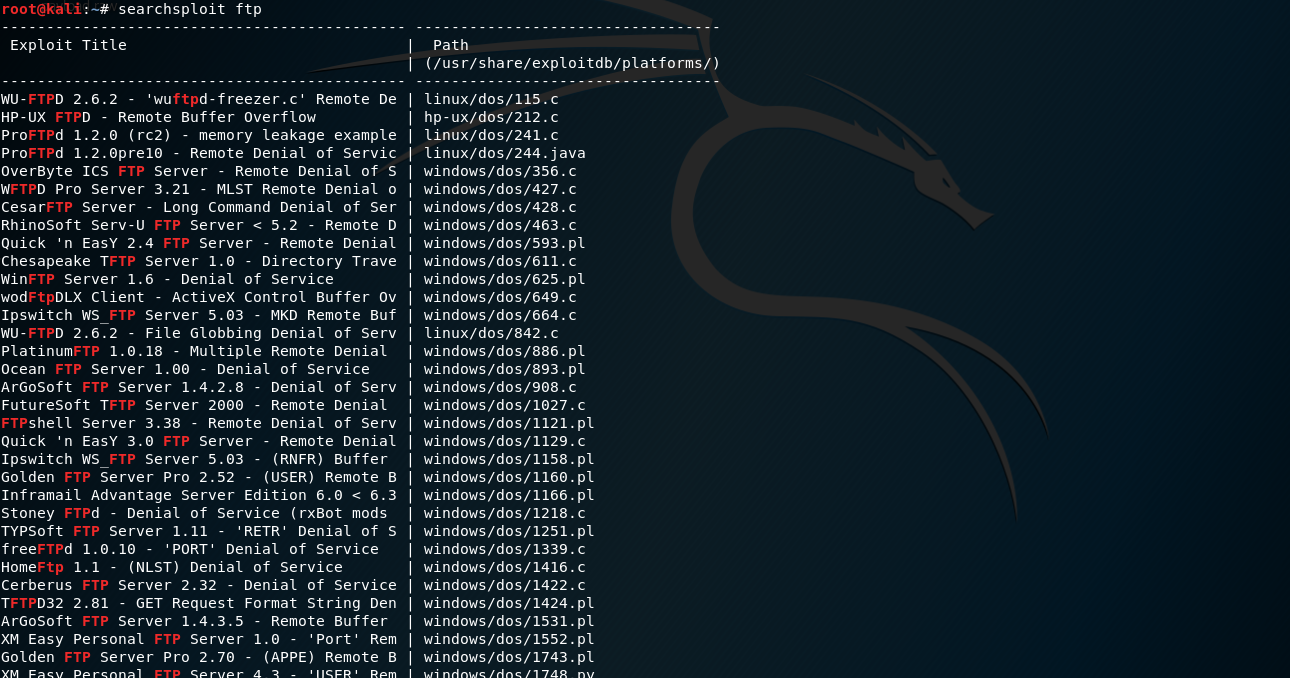
\includegraphics[width=0.8\textwidth]{oui/Ancien/imangeancien/metasploit/searchsploit-ex.PNG}
  \caption{Recherche d'exploit dans la DB communautaire exploit-db}
  \label{fig:exploit-db}
\end{figure}

\noindent Cette commande nous retourne une liste des exploits disponible pour le service FTP. On remarque également que ces exploits sont stockés dans le répertoire \textbf{/usr/share/exploitdb/plateforms}.

\noindent Si on le souhaite, on peut faire une recherche en fonction de la version du service :
\begin{figure}[htp!]
  \centering
  \setlength\figureheight{7cm}
  \setlength\figurewidth{9cm}
  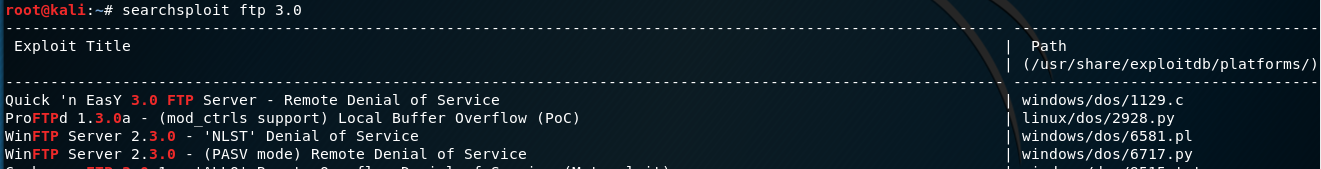
\includegraphics[width=0.8\textwidth]{oui/Ancien/imangeancien/metasploit/searchsploit-ex2.PNG}
  \caption{Recherche en fonction de la version}
  \label{fig:courbe-tikz}
\end{figure}

    \noindent Cela permettra de cibler plus facilement l'exploit à utiliser. Enfin, il faut savoir que tous les exploits présentés avec la commande \textbf{searchsploit} ne sont pas tous des exploits utilisables avec Metasploit. En effet, tous les exploits codés n'ont pas été faits pour Metasploit. On peut y retrouver des exploit en python ou encore en C. Cependant, tous les exploits compatibles avec metasploit auront la mention \textbf{(metapsloit)} dans leur nom lors de la recherche avec \textbf{searchsploit}. 

\subsection{Utilisation des modules et des exploits}

Comme nous l'avons dit en introduction, Metasploit utilise des modules pour fonctionner. Dans cette partie, nous allons voir comment les utiliser dans le cadre d'un audit de sécurité ou sur un CTF. La partie des modules est décomposée en 5 sous-parties qui sont :\\

- \textbf{Exploit}: Un exploit est le moyen par lequel un pentester exploite une faille, un défaut dans un logiciel ou un service. Ainsi, un attaquant peut utiliser un exploit pour attaquer un système d'informations et générer ainsi un résultat que les développeurs n'ont pas pris en compte. Les exploits les plus courants sont le débordement de tampon (buffer overflow), les vulnérabilités Web (injection SQL, défaillances XSS) et enfin les erreurs de configuration dans un logiciel.

- \textbf{Payloads}: Un payload ou charge utile est un code qui sera exécuté par le système. Dans cette partie, on peut y retrouver tout type de payload comme le reverse shell, c'est le fait de créer une connexion depuis la cible vers l’attaquant. De plus, Metasploit permet de regrouper les payloads en fonction du système d'exploitation (OS) de la machine victime.

- \textbf{Encoders}: C'est un module de metasploit permettant d'encoder des payloads ou des shellcode dans le but d'outrepasser la détection antivirus et les IDS. En effet, en encodant plusieurs fois un code malveillant, l'antivirus de la machine cible devra faire beaucoup de calculs avant de détecter le virus. Pour faire ses analyses, un antivirus place le programme à analyser dans une sandbox (machine virtuelle isolée de l'hote) dans laquelle il va faire ses analyses. Cependant, lors d’une analyse régulière du système, l’antivirus devra analyser des milliers de fichiers. Il ne peut pas se permettre de passer trop de temps sur un fichier en particulier.

- \textbf{Nops}: En langage assembleur, NOP est l'abréviation de No Operation. Le NOP permet de garder une taille de payload constante en s'assurant que tout espace non utilisé par un autre code sera toujours valablement exécutable par le processeur. En effet, lors de l'écriture d'un payload ou d'un shellcode, les NOP permettent de régler la problématique des sauts d'instructions en assembleur. Cette partie est utilisée lors de la programmation d'exploit ou de payload pour metasploit.

- \textbf{AUX}: "AUX" correspond aux modules auxiliaires de metasploit. Comme par exemple les scans de ports, de versions de services en utilisant NMAP.

Ce qui peut être très intéressant avec cet outil, c'est de combiner l'utilisation de NMAP et de Metasploit. En effet, NMAP permet de trouver des versions de services. Il nous suffit de chercher de versions vulnérable avec Metasploit. Comme nous l'avons vu précédemment, on peut utiliser la commande \textbf{searchsploit}. Si cela ne suffit pas, on peut chercher des exploits sur le net et les importer dans Metasploit. Pour utiliser un exploit, il suffit de faire la commande \textbf{use exploit/le\_chemin\_de\_l'exploit}. On peut également utiliser \textbf{use} pour utiliser tous les modules de Metasploit tel que le module auxiliaire avec \textbf{use auxiliary/chemin\_du\_programm}.\\

Pour rechercher un exploit directement dans metasploit afin de l'utiliser, on utilise la commande \textbf{search}. Cette commande va chercher tous les exploits disponibles dans Metasploit pour l'argument passé en paramètre.\\ 

\noindent On reprenant l'exemple de la section précédente, on aurait pu faire ceci:

\begin{figure}[htp!]
  \centering
  \setlength\figureheight{7cm}
  \setlength\figurewidth{9cm}
  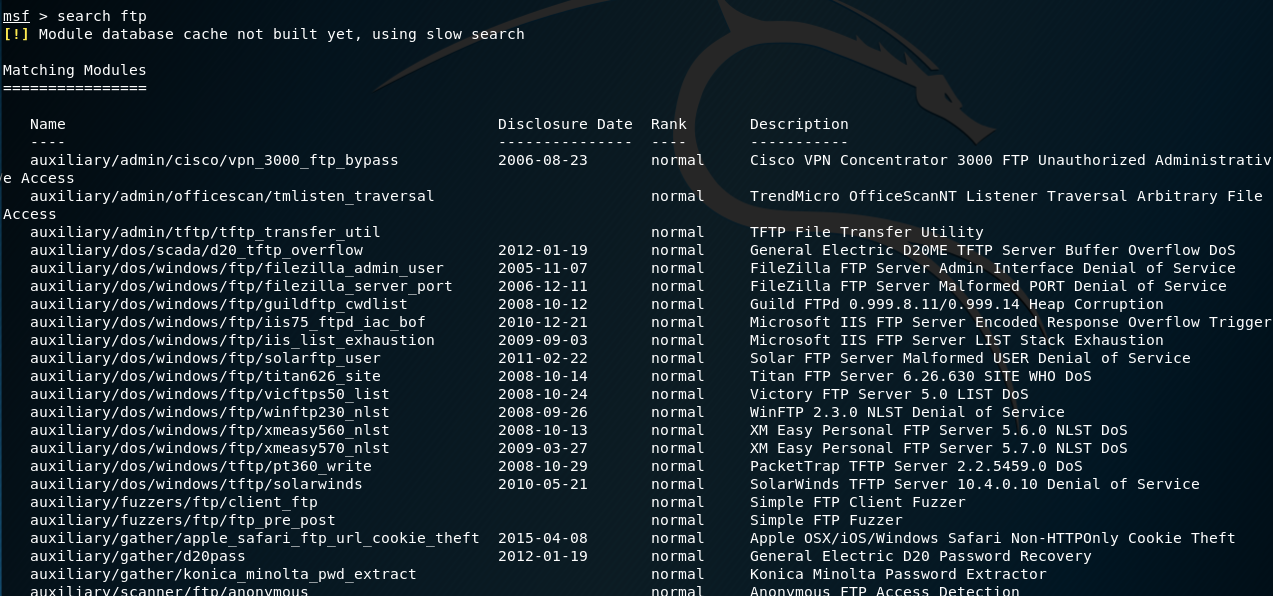
\includegraphics[width=0.8\textwidth]{oui/Ancien/imangeancien/metasploit/search.PNG}
  \caption{Search ftp}
  \label{fig:courbe-tikz}
\end{figure}

Cette capture donne le "chemin" de tous les exploits en rapport avec FTP 3.0.

\subsection{Utilisations}

\subsubsection{Exemple d'utilisation pour exploiter un service}

Pour cette exemple, nous allons voir comment exploiter un service vulnérable avec Metasploit. La machine cible sera une machine metasploitable2 conçu pour être vulnérable à beaucoup d'attaques:

\begin{figure}[htp!]
  \centering
  \setlength\figureheight{7cm}
  \setlength\figurewidth{9cm}
  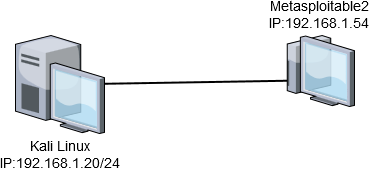
\includegraphics[width=0.5\textwidth]{oui/Ancien/imangeancien/metasploit/schema.png}
  \caption{Schéma de la maquette}
  \label{fig:courbe-tikz}
\end{figure}

\newpage

Il suffit d'utiliser NMAP pour scanner la machine:
\begin{figure}[htp!]
  \centering
  \setlength\figureheight{7cm}
  \setlength\figurewidth{9cm}
  \includegraphics[width=0.8\textwidth]{oui/Ancien/imangeancien/metasploit/nmap.PNG}
  \caption{NMAP dans Metasploit}
  \label{fig:courbe-tikz}
\end{figure}

Ensuite on peut chercher des exploits sur \textbf{vsftpd 2.3.4}:
\begin{figure}[htp!]
  \centering
  \setlength\figureheight{7cm}
  \setlength\figurewidth{9cm}
  \includegraphics[width=1\textwidth]{oui/Ancien/imangeancien/metasploit/ftp.PNG}
  \caption{search vsftpd 2.3.4}
  \label{fig:courbe-tikz}
\end{figure}

On constate qu'il existe un exploit pour effectuer un reverse shell sur la machine. On va donc l'utiliser avec la commande \textbf{use}:

\begin{figure}[htp!]
  \centering
  \setlength\figureheight{7cm}
  \setlength\figurewidth{9cm}
  \includegraphics[width=0.8\textwidth]{oui/Ancien/imangeancien/metasploit/ftp5.PNG}
  \caption{use exploit}
  \label{fig:courbe-tikz}
\end{figure}

\noindent On peut utiliser la commande \textbf{show options} pour voir les options de cet exploit:

\begin{figure}[htp!]
  \centering
  \setlength\figureheight{7cm}
  \setlength\figurewidth{9cm}
  \includegraphics[width=0.8\textwidth]{oui/Ancien/imangeancien/metasploit/ftp3.PNG}
  \caption{Show options}
  \label{fig:courbe-tikz}
\end{figure}

\newpage
On constate que nous devons renseigner un \textbf{RHOST}(Remote Host) qui correspond à la machine victime. On utilise la commande \textbf{set RHOST} pour éditer une option. Pour cet exemple, nous allons faire \textbf{set RHOST 192.168.1.54}. Une fois fait, on peut regarder à nouveau les options : 


\begin{figure}[htp!]
  \centering
  \setlength\figureheight{7cm}
  \setlength\figurewidth{9cm}
  \includegraphics[width=0.8\textwidth]{oui/Ancien/imangeancien/metasploit/ftp3.PNG}
  \caption{Set RHOST}
  \label{fig:courbe-tikz}
\end{figure}

On constate que le champ \textbf{RHOST} a bien été renseigné. On peut à présent lancer l'exploit avec la commande \textbf{exploit}:

\begin{figure}[htp!]
  \centering
  \setlength\figureheight{7cm}
  \setlength\figurewidth{9cm}
  \includegraphics[width=1\textwidth]{oui/Ancien/imangeancien/metasploit/ftp4.PNG}
  \caption{Lancement de l'exploit}
  \label{fig:courbe-tikz}
\end{figure}

On s'aperçoit que l'exploit s'est bien exécuté sur la machine cible. Nous avons donc un reverse shell sur la machine distante.

\subsubsection{Récupération d'utilisateurs d'un serveur SMB}
Dans le cas d'un CTF qui utilise un serveur Samba par exemple, Metasploit peut être très utile pour énumérer la liste des utilisateurs du serveur Smb. Metasploit possède un module de scan permettant de faire cela. Il se trouve dans \textbf{auxiliary/scanner/smb} (voir \textbf{figure \ref{fig:smb-enum}})\\

\begin{figure}[h]
  \centering
  \setlength\figureheight{7cm}
  \setlength\figurewidth{9cm}
  \includegraphics[width=0.8\textwidth]{oui/Ancien/imangeancien/msf_smb_enum.PNG}
  \caption{Utilisation du module smb\_enum}
  \label{fig:smb-enum}
\end{figure}

Il nous suffit de renseigner le champ "rhosts" qui correspond à l'adresse IP de la machine victime. Ensuite on tape "exploit" pour lancer le module. En quelques secondes, nous récupérons un utilisateur nommé "helios" qui est un utilisateur du serveur Samba.\\

On peut également récupérer le mot de passe avec une attaque par dictionnaire disponible avec un autre module nommé \textbf{smb\_login} comme indiqué dans la \textbf{figure \ref{fig:attaque-smb-dic}}

\begin{figure}[]
  \centering
  \setlength\figureheight{7cm}
  \setlength\figurewidth{9cm}
  \includegraphics[width=0.9\textwidth]{oui/Ancien/imangeancien/msf_smb_pass.PNG}
  \caption{Attaque par dictionnaire smb}
  \label{fig:attaque-smb-dic}
\end{figure}
Enfin, il faut renseigner l'utilisateur avec lequel on veut trouver le mot de passe ainsi qu'un dictionnaire à utiliser. Dans notre cas, nous allons utiliser le dictionnaire "rockyou" qui est un dictionnaire comprenant 14.344.392 lignes (voir \textbf{figure \ref{fig:smb-dic-2}})\\

\begin{figure}[]
  \centering
  \setlength\figureheight{7cm}
  \setlength\figurewidth{9cm}
  \includegraphics[width=0.9\textwidth]{oui/Ancien/imangeancien/msf_smb_pass2.PNG}
  \caption{Attaque par dictionnaire smb}
  \label{fig:smb-dic-2}
\end{figure}

Metasploit a trouvé le mot de passe de l'utilisateur "helios" qui était "qwerty". On peut donc se connecter au serveur SMB avec notre utilisateur:

\begin{figure}[h]
  \centering
  \setlength\figureheight{7cm}
  \setlength\figurewidth{9cm}
  \includegraphics[width=0.9\textwidth]{oui/Ancien/imangeancien/msf_smb_pass3.PNG}
  \caption{Connexion au serveur SMB}
  \label{fig:courbe-tikz}
\end{figure}